\section{Estrazione e classificazione delle facce}
\label{sec:face_extraction}

\subsection{Grafo planare embedded e struttura dati Half-Edge}
\label{subsec:half_edge}

Dopo che abbiamo ricostruito le fessure tra i muri, la geometria è rappresentata dagli stessi vertici (univoci) ma con degli archi in più. L'insieme di tutti gli archi sono etichettati come \texttt{WALL}, \texttt{DOOR} o \texttt{WINDOW}.
A partire da questa rappresentazione, l'obiettivo è costruire un grafo planare embedded da cui estrarre le facce poligonali, che costituiranno la base per la successiva triangolazione ed estrusione.

Un grafo planare è un grafo che \emph{può} essere disegnato su una superficie piana (ad esempio un foglio di carta) senza che i suoi archi si incrocino; non tutti i grafi sono planari. Un grafo planare embedded (o grafo piano) è invece un grafo planare che è stato \emph{effettivamente} mappato su un piano, in modo tale che due archi non si intersechino se non nei loro vertici comuni.
\begin{figure}[htbp]
	\centering
	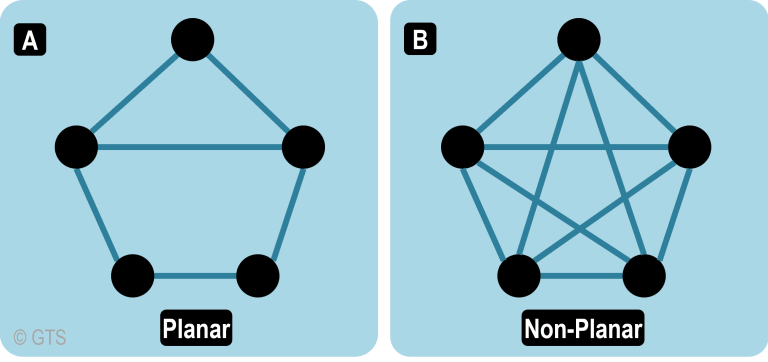
\includegraphics[width=1\textwidth]{images/02_geometry_processing/planar_non_planar_graphs.png}
	\caption{Grafo planare e non planare}
	\label{fig:planar_non_planar_graphs}
\end{figure}

Un grafo planare rettilineo (\emph{Planar Straight-Line Graph}, PSLG) è un grafo planare embedded i cui archi sono rettilinei anziché curvi. 

Esistono tre strutture dati ben note per rappresentare un PSLG: \texttt{Winged-Edge}, \texttt{Half-Edge} e \texttt{Quad-Edge}. In questo lavoro si è scelto di adottare la struttura Half-Edge \cite{yin2024halfedge, uiuc2024halfedge}, messa a disposizione direttamente dalla libreria CGAL utilizzata per la costruzione del grafo.

La struttura dati Half-Edge, chiamata anche \emph{doubly-linked edge list}, è una rappresentazione a grafo comunemente utilizzata in computer grafica e geometria computazionale per memorizzare mesh poligonali. Una mesh poligonale può essere vista come un grafo, costituito da vertici, archi e facce, ciascuna definita come un ciclo ordinato di vertici.

La struttura Half-Edge memorizza esplicitamente ogni arco come una coppia di archi orientati in direzioni opposte, detti \emph{twin} (gemelli). Ogni arco mantiene un riferimento al proprio gemello, oltre ai riferimenti all'arco precedente e successivo lungo la stessa faccia. Ogni vertice memorizza la propria posizione e un riferimento a uno degli archi uscenti da esso; ogni faccia memorizza a sua volta un riferimento a uno degli archi che la delimitano. La struttura risulta quindi composta da tre insiemi di record: vertici, facce e archi.

\begin{figure}[htbp]
	\centering
	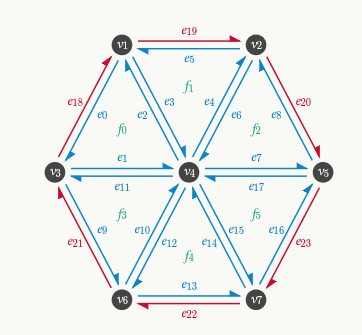
\includegraphics[width=0.5\textwidth]{images/02_geometry_processing/half-edge.png}
	\caption{Visualizzazione Half-edge}
	\label{fig:visualization-half-edge}
\end{figure}

Una volta costruito l'Half-Edge, il nostro output non è più un semplice elenco di segmenti, ma una raccolta di poligoni 2D (facce) distinti ed espliciti. A partire da questa rappresentazione è possibile procedere con l'estrazione e la classificazione delle facce, descritte nella sezione successiva.

\subsection{Costruzione del PSLG con CGAL}
\label{subsec:pslg_cgal}

Per implementare la struttura dati descritta, si è scelto di utilizzare la libreria CGAL \cite{cgal}, che fornisce la classe \texttt{CGAL::Arrangement\_2}. Questa classe rappresenta un PSLG e fornisce accesso a vertici, half-edge e facce tramite appositi iteratori.

La costruzione dell'arrangement avviene passando a CGAL la lista dei vertici univoci (prodotti dalla fase di vertex snapping) e la lista degli archi etichettati. CGAL restituisce un oggetto \texttt{Arrangement\_2} che contiene la lista delle facce.
\newpage

\begin{minted}[frame=single]{cpp}
CGAL::Arrangement_2 build_arrangement(
  const std::vector<glm::dvec2>& vertices, 
  const std::vector<Edge>& edges
);

std::vector<Face> extract_faces(const Arrangement& arr);
\end{minted}

Una faccia è rappresentata come:
\begin{minted}[frame=single]{cpp}
class Face
{
  std::vector<glm::dvec2> vertices;
  std::vector<SegmentLayer> edge_layers;
  FaceType type;
};
\end{minted}


È importante notare che l'arrangement include sempre una faccia illimitata (\texttt{unbounded\_face()}), che rappresenta l'esterno del disegno e che deve essere esclusa dalla classificazione.

\subsection{Classificazione delle facce}
\label{subsec:face_classification}

Una volta costruito l'arrangement, è possibile iterare sulle facce e classificarle in base agli archi. 

La classificazione si basa sull'etichetta assegnata: una faccia è classificata come \texttt{DOOR} se e solo se ha esattamente 4 archi, di cui 2 etichettati come \texttt{DOOR} e 2 come \texttt{WALL}; una faccia è classificata come \texttt{WINDOW} se e solo se ha esattamente 4 archi, di cui 2 etichettati come \texttt{WINDOW} e 2 come \texttt{WALL}; una faccia è classificata come \texttt{WALL} se tutti i suoi archi sono etichettati come \texttt{WALL}; tutte le altre facce sono classificate come \texttt{FLOOR} (pavimento). Se il modello contiene più stanze, ciascuna di esse sarà rappresentata da una faccia \texttt{FLOOR} separata.

\begin{figure}[htbp]
	\centering
	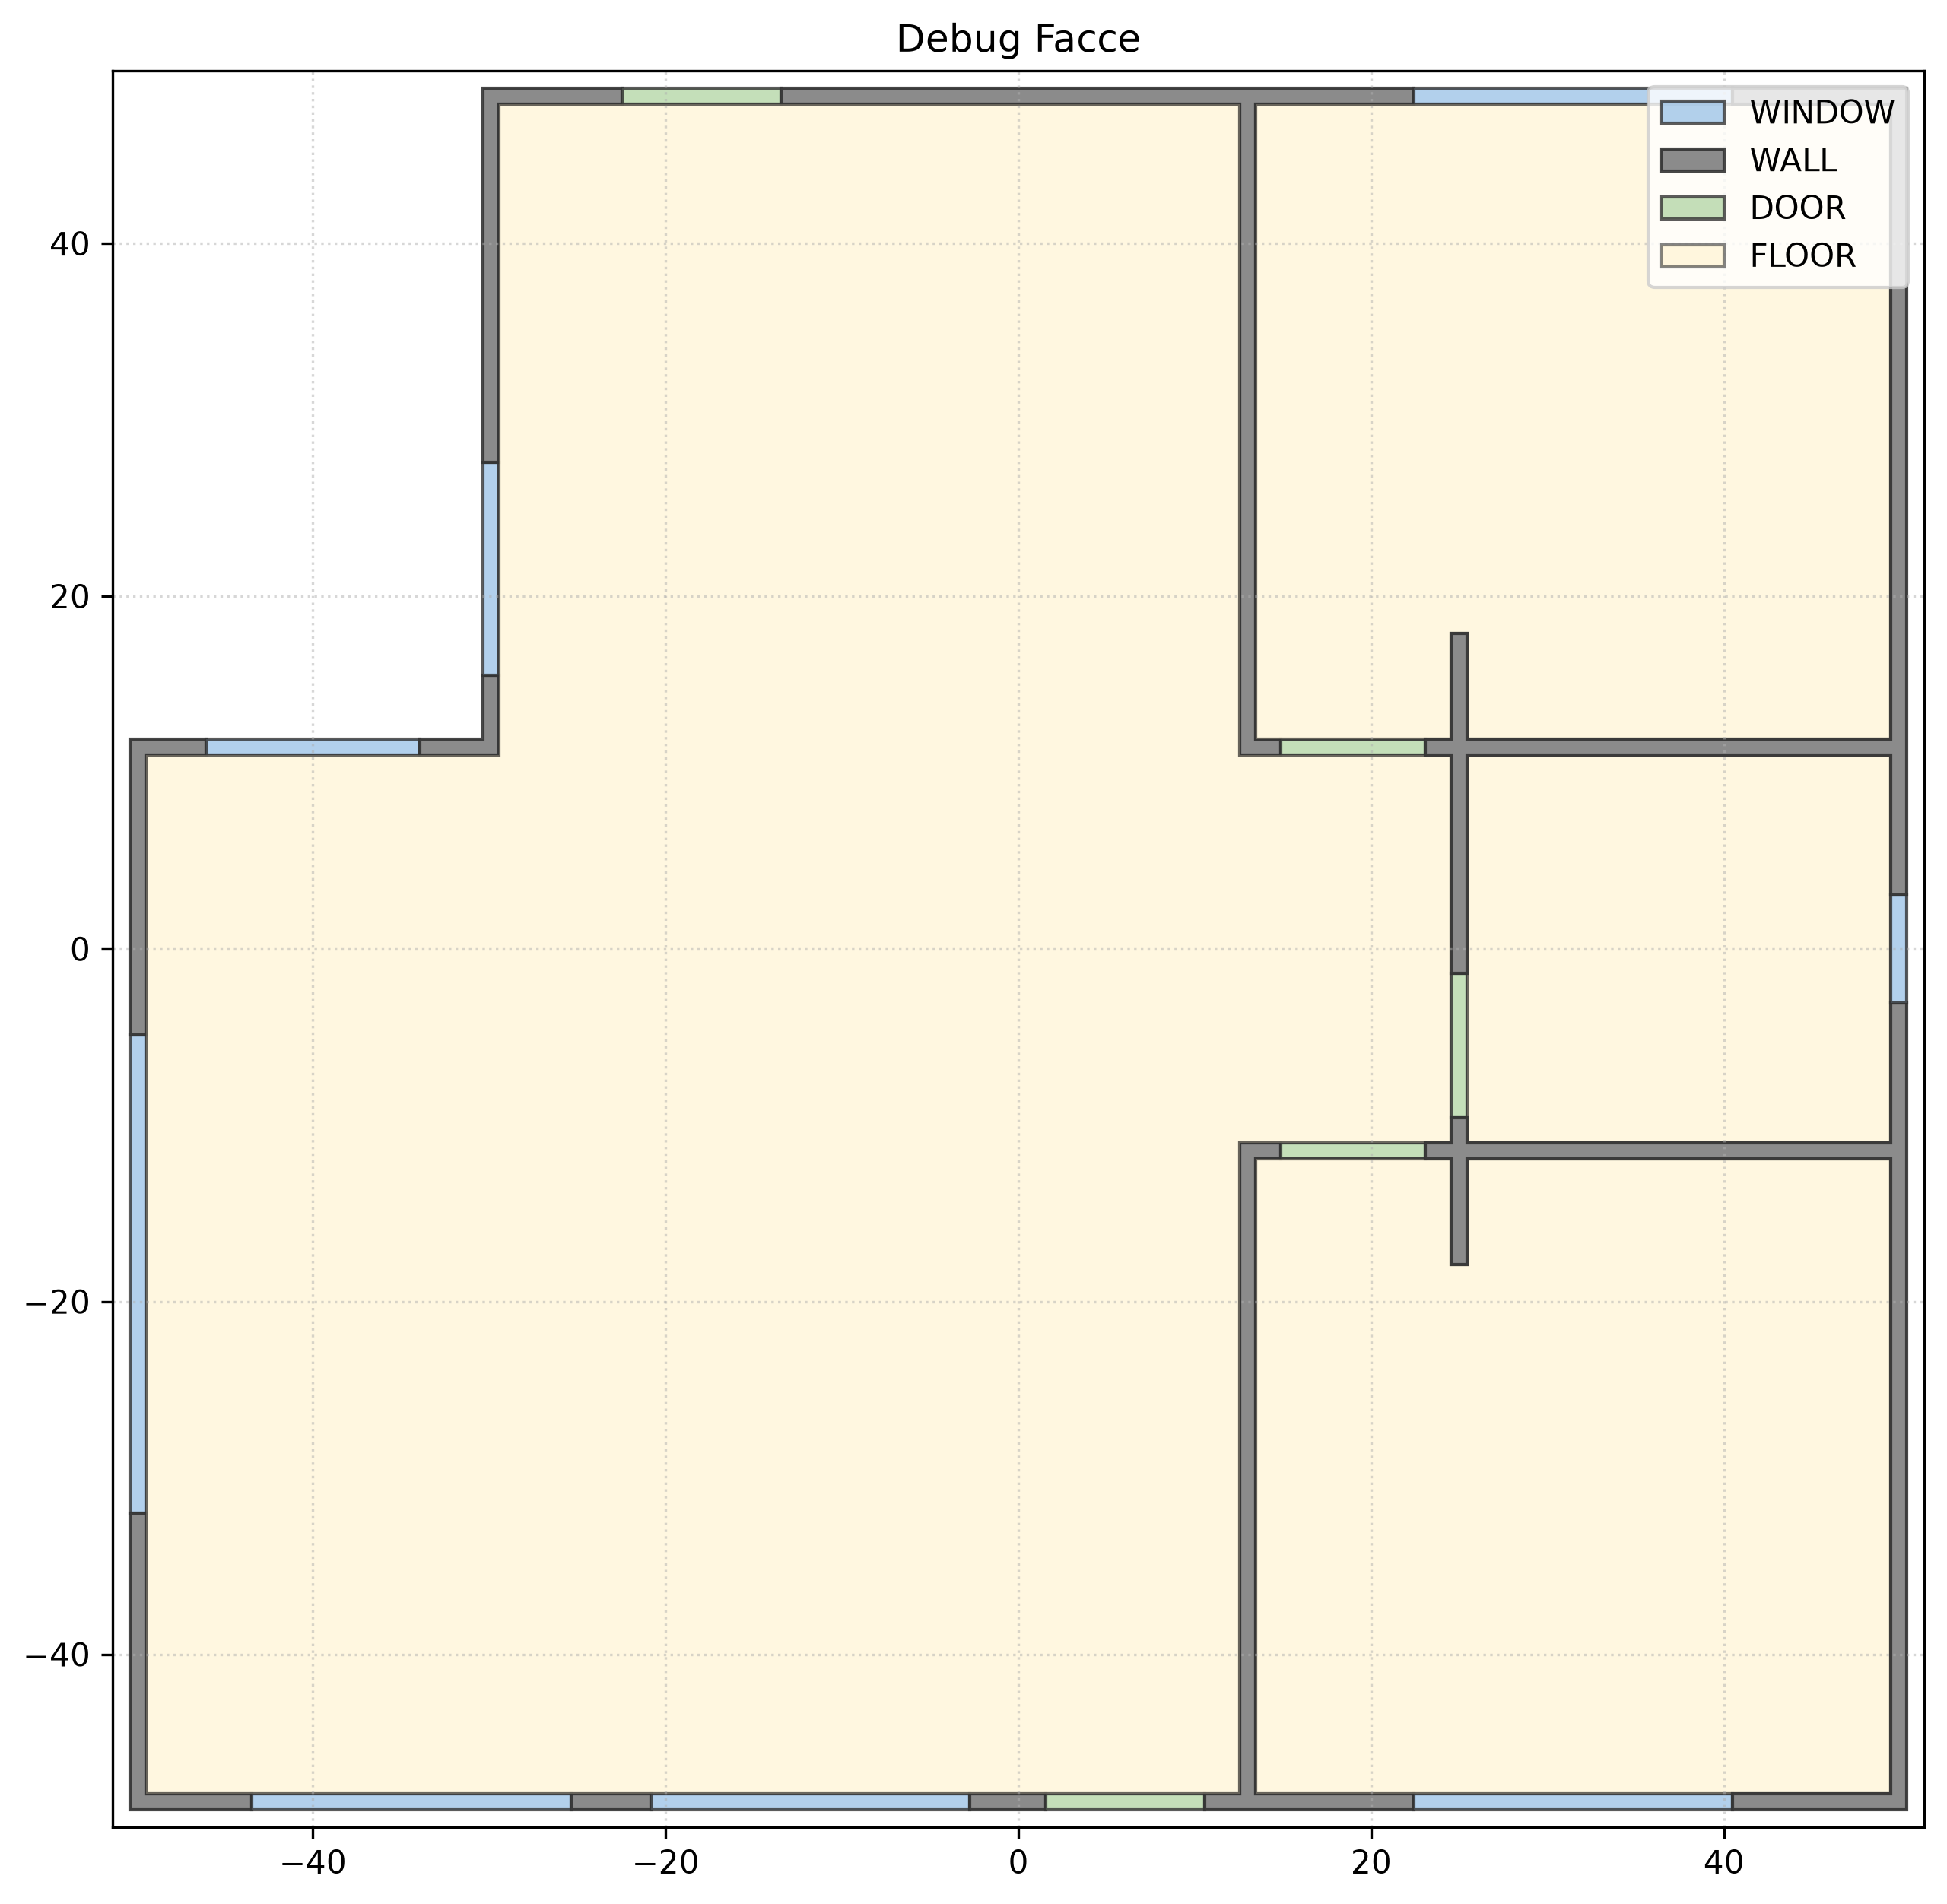
\includegraphics[width=0.75\textwidth]{images/02_geometry_processing/faces.png}
	\caption{Visualizzazione facce}
	\label{fig:faces}
\end{figure}

La classificazione è fondamentale perché l'estrusione viene effettuata in modo differenziato a seconda del tipo di faccia, come vedremo successivamente.

